\documentclass[12pt]{article}
\usepackage{graphicx}
\usepackage{footnote}
\usepackage{inputenc}
\usepackage{setspace}

\begin{document}

\begin{titlepage}
    \title{Collecting Source Code Samples For Sociolinguistic Research}
    \author{Steven Deutekom \\ University of Lethbridge}
    \maketitle
    \thispagestyle{empty}
\end{titlepage}


\pagenumbering{roman}

% Table of Contents
\newpage
\tableofcontents

% List of figures/tables
\newpage
\listoffigures
\listoftables

% Introduction %%%%%%%%%%%%%%%%%%%%%%%%%%%%%%%%%%%%%%%%%%%%%%%%%%%%%%%%%
\newpage
\doublespacing
\pagenumbering{arabic}
\section{Introduction}
% What are we doing?
The goal of this project is to collect source code samples from individual authors from various online sources. It requires finding samples that have certain sociolinguistic characteristics such as gender, region, and experience. In addition to sociolinguistic characteristics, it is necessary that the samples are the work of only a single author. Data that meets these needs is being collected and used to create a dataset with information on authors and their source code.

% Why are we doing it?
The collected data will be used for sociolinguistic research into how people use programming languages. Current and future University of Lethbridge students will use this research to learn how sociolinguistic characteristics affect how programmers write code. Previous research was conducted with a small dataset of student programs \cite{Naz2015} \cite{Rafee2017}. This new dataset will contain many samples from a larger set of programmers.

% What is coming in this documents?
The document is broken into three main sections. Each section details one of the sources that was used to collect data. First, the collection methods used to gather source code from GitHub. Then, the methods used to collect source code from Codeforces. Lastly, the methods that were used to add gender data to the samples collected.

Each section introduces the sources and collection methods. Then it discusses the pros and cons of the source. Next an overview of the process of collecting data is given, with diagrams to help visualize it. Following this a more in depth technical examination of the collection process takes place. An overview of the data that is collected will be given along with a table showing the data types and Database schemas. Finally, any technical more technical issues that were encountered will be discussed.

To conclude there will be some final thoughts on the projects. This will include a summary of threats to the validity of the data will be given. It will then finish with some discussion on ways to expand on the data in the future if desired.


% GitHub %%%%%%%%%%%%%%%%%%%%%%%%%%%%%%%%%%%%%%%%%%%%%%%%%%%%%%%%%%%%%%%
\section{Collecting Source Code From GitHub}


%& Introduction to the sources being used
\subsection{Data Sources}
\subsubsection*{GitHub}
GitHub is one of the largest online code sharing/hosting website on the internet with over 36 million users and over 100 million repositories \cite{WEBSITE:Git1}. It has an API that allows access to information on users, repositories, commits, and more. Source code hosted in public repositories is available for anyone to freely access or use in projects. Data on users, as well as source code is collected from GitHub and added to the database. Two methods are used for this. The first looks at commit data and collects changes to files. The second looks at projects and collects full files of source code. Both support the goal of adding single author source code samples to the database.

\subsubsection*{GhTorrent}
GhTorrent is an offline database of data obtained from the GitHub API \cite{Gousi13}. It contains large quantities of data on GitHub users, projects, commits from as far back as 2012. This data is being collected to support research on software repositories and is available to the public for other research on GitHub. This source is used to collect information on GitHub commits and projects. This information is used to decide which projects and commits to try to collect source code samples for from GitHub. More information is available on the GhTorrent website\footnote{http://ghtorrent.org}.

\subsubsection*{Google BigQuery}
Google BigQuery is a part of the Google Cloud Platform. It allows the storage and querying of datasets online. These datasets and query results can be connected to other google cloud services and also downloaded. The GhTorrent dataset is accessible on BigQuery. Queries on the GhTorrent dataset are made  using and refined using BigQuery in order to find information on the desired commits and projects.


%% Pros and Cons of each along with steps taken to try and overcome any issues.
\subsection{Pros And Cons}
\subsubsection*{GitHub}
\begin{itemize}
    \item The popularity of GitHub means that there is a large amount of source code and data available. This means one can get a reasonable amount of data on even very specific searches.

    \item It's api is full featured and well documented. It can be used to find any information that is available on the website. Except source code which must be obtained in other ways.
    
    \item The nature of the platform makes all public code freely available for anyone to access within the platform. This is outlined in the GitHub terms of service (reference). However, without and open source license source code is still the sole property of the author and cannot be shared or published without their permission.

    \item GitHub is often used for collaboration. It is not always easy to tell wether source code has a single author, but there are contributor lists and other tools that can help \cite{Yang2017}\cite{Matyukhina2019}. However, results from the these tools might not be accurate when used on projects that were added to GitHub long after being stated. It is also possible for code in a repository to be taken from a 3rd party source like libraries, extensions, or freely available code samples.

    \item A Rate limit of 5000 calls per hour is imposed on the GitHub API. By collecting the initial data from GhTorrent the number of API calls is reduced. It is not hard for a process to use up this limit in much less time than 1 hour. If a process will use up the limit it is necessary to have it keep track of time and wait for the API to reset every hour.

    \item When collecting code from commits the changes can be scattered around a file. It is not very useful to have 30 lines of code from an author if those 30 lines are not connected to one another. It is possible to identify changes that are part of a newly added file. This ensures that all the changes represent a single piece of code. One of the issues with this is that newly added files are often not complete.
\end{itemize}

\subsubsection*{GhTorrent}
\begin{itemize}
    \item The GhTorrent database is a massive database of GitHub metadata. Accessing GitHub metadata using GhTorrent can make it much easier to know what kind of data is available on GitHub.
    
    \item Because the GhTorrent database is so big it would be difficult to store it locally. Queries on a database of this size would be slow without good hardware. So for most people access must be through another source like Google BigQuery. 
\end{itemize}

\subsubsection*{Google BigQuery}
\begin{itemize}
    \item BigQuery is run with Googles code platform. The hardware used to process queries will run queries on the GhTorrent database much faster than the hardware most people have access to.

    \item Because BigQuery is part of the Google cloud platform it requires a google account to use. There are also limits on the amount of data that can be queried each month and limits on how much data a person can store. It is possible to increase these limits with payment if needed.

    \item BigQuery also has a limit on how many rows of data can be downloaded at once. This can make it more time consuming to download the results of large queries. Details of this process can be found below.
\end{itemize}


%% High level overview of the process w/ diagrams
\subsection{Process Overview}

%%% Ght and BigQuery process
\subsubsection*{GhTorrent and Google BigQuery}
SQL queries are made on the GhTorrent dataset via BigQuery. These queries are refined until the results are satisfactory. Once desired results are obtained they can be saved or downloaded. It is often best to save the results of a large query and then sample it with another query. These sample results can then be split and downloaded. If the results were split they can be recombined before being processed by one of the collection methods for GitHub.

% Process Diagram
\begin{figure}[t]
    \centering
    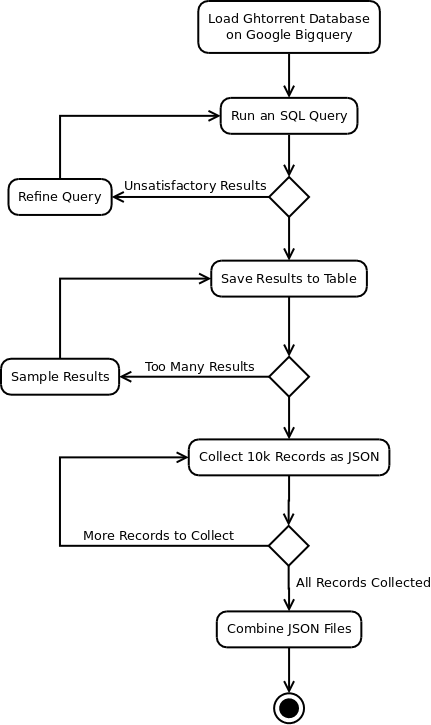
\includegraphics[height=10cm]{diagrams/ght_process.png}
    \caption{Getting Data From GhTorrent via BigQuery}
\end{figure}

%%% Git projects process
\subsubsection*{Collecting Git Projects}
The list of GitHub project data collected from GhTorrent is loaded and each entry is processed. If the project referenced by an entry is valid its repository is cloned locally. Then every valid folder is searched to find valid single author files. All valid files are then processed by having their source code collected and further validated. If the source code is valid it is added, along with user and project information, to the database. Once a project is finished being processed the cloned repository is removed.

% Process Diagram
\begin{figure}[t]
    \centering
    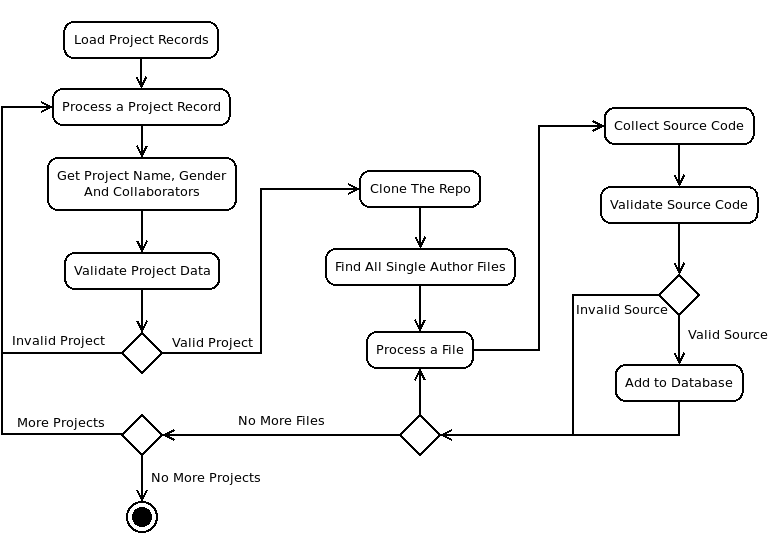
\includegraphics[height=8cm]{diagrams/projects.png}
    \caption{Getting GitHub Project Source Code}
\end{figure}

%%% Git commits process
\subsubsection*{Collecting Git Commits}
The list of GitHub commit data collected from GhTorrent data is loaded and each entry is processed. First the entry's commit information is requested from the GitHub API. If this information is available, all the files that have changes are validated. If a set of changes is valid it is collected and has any extra symbols that were added by GitHub removed. Then the source code is added, along with user, project, and commit information, to the database.

% Process Diagram
\begin{figure}[t]
    \centering
    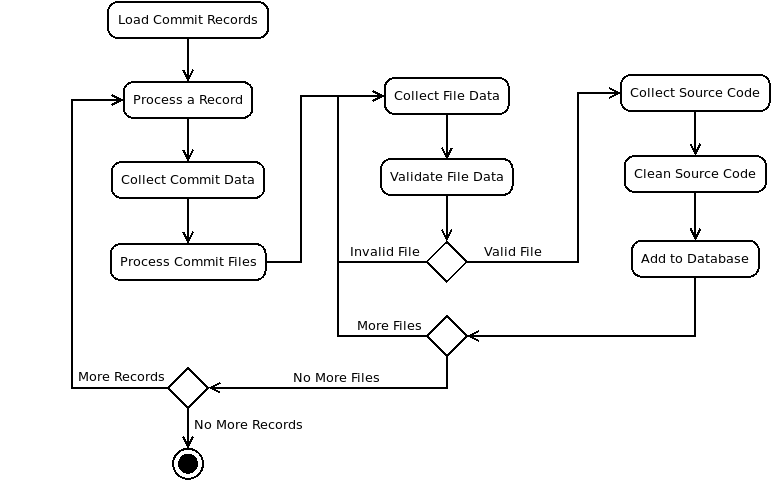
\includegraphics[height=7.5cm]{diagrams/commits.png}
    \caption{Getting GitHub Commit Source Code}
\end{figure}


%% Discussion of each subprocess
\subsection{Process Details}

%%% Ght and BigQuery process
\subsubsection{GhTorrent and Google BigQuery}

\subsubsection*{Process}
The GhTorrent database is accessed via BigQuery\footnote{https://bigquery.cloud.google.com/dataset/ghtorrent-bq:ght}. From here SQL queries are made on the database to find data for users, projects, and commits. The exact queries depend on which collection method is being used. Both collection methods collect only one programming language at a time, so queries filter out all but the desired language. Since research is being done on region records where country code is NULL are filtered out. These queries run quite quickly and are refined until only the desired results are obtained.

Results are saved to a table in the users personal datasets. A dataset and table can be created to save the results of any query. Though there are only 10GB available in the free tier. Once saved if the results are too big then they are randomly sampled to reduce their size. To build our dataset approximately 150,000 records per programming language were collected. This allowed 6-10,000 users who's combined samples had 300 or more lines of code. When a sample is taken it is saved to a table so it can be downloaded within the constraints of BigQuery.

The final table of results is able to be downloaded with a maximum of 10,000 rows at a time. The table is queried with SQL that allows it to be broken up into pieces that are downloaded as json files. Once each section of 10,000 records has been downloaded as json files they are combined with a into one or more data files. These resulting data files are formatted so they are can be parsed by Python3's json library and iterated over by the GitHub processes.

\subsubsection*{Data}
The downloaded json files have each row of the query represented as a json record on it's own line. Each record is a collection of key value pairs, where the key is the column name. Because the records are not contained in a list they must be pre-processed before they can be loaded with Python3's json library. This is taken care of by the script that combines the downloaded results into one or more data files. Once processed each record is an entry in a list that can be iterated over. The columns in each record can be accessed by their corresponding column name from the SQL query that created them. The Fields for a user's company, state, city, and location are allowed to be NULL for our collection processes. The fields necessary for each process differ and will be described in the process's Data section.

%%% Git projects process
\subsubsection{Collecting Git Projects}
% Removed this introduction, but should there be a section devoted to the pros and cons of each process, and maybe describing the goals of that process?
\subsubsection*{Process}
First a file containing a list of project records collected from the GhTorrent dataset via BigQuery is loaded. For each project record an attempt is made to add the users full name and their gender. The name is collected by using the GitHub API for user information. If there is a full name the first name is extracted and passed to a gender checking function. This function calls a gender API to obtain gender information. If name or gender cannot be added to the project record the process moves on to the next record. If both name and gender are found they are added to the record. Next, a call to the GitHub API is made to get a list of contributors to the project. If there are more than one contributors to a project the process continues with the next project record.

If name, gender, and contributors are successfully added to the record the script clones the project repository into a temporary directory. The repository is searched to find all files that were only contributed to by the project owner. To attempt to limit the collection of files added from other sources some directories are excluded from the search. For example, lib, ext, and samples and other variations of these directory names are ignored \cite{Matyukhina2019}. There is also a list of files that are not included. This depends on the programming language. For example {\_\_}init{\_\_}.py files in Python packages. Files that are not ignored are checked to make sure they have an extension that matches the programming language being collected. The files are also checked with git blame to determine if more than one author contributed to them \cite{Wisse2015}. Because the record only contains information on the repository owner collected only files where the author is the same as the repository owner are collected. When all files have been checked a list of file paths for the valid files is returned.

The source code is collected from each file in the list of valid files. The number of lines in the source code is counted. Any file with less than 10 lines or more than 1000 lines is ignored. Valid source code, the filename, and number of lines to the project record are collected together. A hash of the file path in the repository is made to be used along with the project id to create a unique key to prevent duplicate files from being collected. Once all this information has been collected it is added, along with all information contained in the project record, to the database. After all the valid files have been added to the database the process continues for the next project record.

When all project records are processed or a given limit for number of records to process is reached the process ends. Details on the range of records processed and the success rate for project and added files are displayed.

\subsubsection*{Data}
Data is collected for the user, project, and each file. The required user information collected is GitHub login, full name, country code, gender, and gender probability. All of these are collected as strings except for gender probability which is a number between 0.0 and 1.0. All of these fields will be present on any project record that is stored in the database. Other data collected on the user includes company, city, state, location, type, and time created. All of these are strings except for the time created which is a time stamp. These fields are not required for collection and can NULL. The time stamp will most likely always be there even though it is not required.

The project information collected is project name, GitHub API url, programming language, and creation time. These fields will always be present when making queries on the GhTorrent dataset vis BigQuery, but only the url and programming language are required. The fields are all strings except the creation time which is a time stamp. The programming language is the primary programming language used on the project and the project repository may contain files of other types.

File information is gathered during the processing of a project record. It include the source code, number of source code lines, file path within the repository, and a hash of the file path. All these fields are strings except for the source code lines which is an integer. These fields are required for a sample to be added to the database.

\begin{table}[t]
    \begin{center}
        \caption{GitHub Project's Data Fields}
        \label{tab:git_data}
        \begin{tabular}{|l | c | c |}
            \hline
            \textbf{Field} & \textbf{Type} & \textbf{Required}\\
            \hline
            Login & String & Yes\\
            Fullname & String & Yes\\
            Gender & String & Yes\\
            Gender Probability & Float & Yes\\
            Company & String & No\\
            User Created & String & No\\
            User Type & String & No\\
            Country Code & String & Yes\\
            State & String & No\\
            City & String & No\\
            Location & String & No\\
            \hline
            Project Url & String & Yes\\
            Project Name & String & No\\
            Programming Language & String & Yes\\
            Project Created & String & No\\
            \hline
            File Hash & String & Yes\\
            File Name & String & Yes\\
            File Contents & String & Yes\\
            File Lines & Int & Yes\\
            \hline
        \end{tabular}
    \end{center}
\end{table}

\subsubsection*{Technical Issues}
There are a number of calls to external services while collecting samples from GitHub projects. It can be difficult to properly handle all of the possible responses and connection issues. This makes it difficult to automate the process in a way that it can be guaranteed to run for long periods unattended.

In order to process each file for its contents and check the number of contributors it is necessary to clone the project repository. If a project is large or has media files it can take a long time to download. This can slow down collection and use a large amount of bandwidth. Many projects are cloned and do not result in any files being collected. By filtering projects for single contributors there are fewer large projects being collected, but it is not fool proof.


%%% Git commits process
\subsubsection{Collecting Git Commits}

\subsubsection*{Process}
First a file of commit records collected from the GhTorrent dataset via BigQuery is loaded. Like the GitHub projects collection an attempt is made to collect information for name and gender. If found this information is added to the commit record. If no name and gender information is found the process continues with the next commit record.

For each commit record a request is made to the GitHub API to collect the details of the commit. The response to this request contains information on every file that was a part of the commit. Each file has a file name and is marked as being modified or added. It also has the text for each line that was changed. Changes to modified files can be spread around the file and it is not clear if a whole line was changed or just some parts of it. For this reason only files marked as added are collected. This way the code collected was all guaranteed to be added by the author of the commit. It is still difficult to be sure that the commit author wrote the new file before adding it.

Each file in the commit data response is validated. As stated above it must be an added file. It must also have more than 10 changes, which corresponds to 10 lines of source code. The file name is also examined to make sure it has an extension that is for the programming language being collected. If a file meets all of these conditions then it's source is collected.

The commit data response has some some text added to it that is not part of the source code. A header is added that contains information on the number of additions and deletions to the file during this commit. This header is removed from the source code. Also, because the changes show the differences between a file and its previous iteration each line has a + or - at the start. Since only added files are collected all lines are preceded by a +. All of these are also cleaned out of the source code before adding it to the database.

The cleaned source code is collected along with the number of file changes. These are added to the database with all the information from the commit record.
Once each valid file in the commit response is added to the database the process continues with the next commit record.

When all commit records are processed or a given limit for number of records to process is reached the process ends. Details on the range of records processed and the success rate for commits and added files are displayed.

\subsubsection*{Data}
Data is collected for the user, project, commit, and each file. The user and project information is the same as the GitHub projects process. The information collected for the commit is commit SHA, and creation time. The SHA is a unique string identifier for the commit generated by GitHub and the creation time is a time stamp indicating when the commit was made. Both are required information and should be present in the commit record collected from the GhTorrent dataset via BigQuery.

The file information is also the same as the projects process except that file lines is replaced with file changes and the status of the file is collected. The changes are an integer and the status is a string. Both are collected when processing the commit data response from the GitHub API and they are required in order to add a source code sample to the database.

\begin{table}[t]
    \begin{center}
        \caption{GitHub Commit's Data Fields (that differ from Table 1)}
        \label{tab:commit_data}
        \begin{tabular}{|l | c | c |}
            \hline
            \textbf{Field} & \textbf{Type} & \textbf{Required}\\
            \hline
            Commit Sha & String & Yes\\
            Commit Created & String & No\\
            File Sha\footnote{Instead of File Hash} & String & No\\
            File Changes\footnote{Instead of File Lines} & Int & Yes\\
            \hline
        \end{tabular}
    \end{center}
\end{table}

% Codeforces %%%%%%%%%%%%%%%%%%%%%%%%%%%%%%%%%%%%%%%%%%%%%%%%%%%%%%%%%%%
\section{Collecting Source Code From Codeforces}


%% Introduction to the source being used %%
\subsection{Data Source}
\begin{sloppypar}
Codeforces is a website that hosts programming contests and allows users to submit solutions to a large database of programming contest problems. The operators of the site describe it as a social network for people interested in contest programming and as a platform for hosting programming contests \cite{WEBSITE:CF1}. Submissions submitted by a user available on the user's profile. The website has an API that can be used to collect user and submission information, but not to collect submission source code. However, the source code for user submissions is accessible through their profile. Codeforces is one of the more popular sites available for contest programming and regularly hosts contests. As of May 2019 there were over 180k users that had participated in at least one ranked contest.
\end{sloppypar}

%% Pros and cons of collecting from codeforces along with steps taken to try and overcome any issues. %%
\subsection{Pros And Cons}
\begin{itemize}
    \item Making the source code of user's solutions available for anyone to view is not common with programming contest websites. This makes Codeforces a valuable resource for this kind of programming.
    
    \item Codeforces is very popular among users in Eastern Europe and parts of Asia. There is more regional diversity than sites like GitHub that are more popular in North America.
    
    \item Users that participate in ranked contests have a rating that is adjusted based on their performance. This makes it possible to get an idea of a programmer's skill and experience.
    
    \item Users that choose to enter one have a first name. This makes it easier to use the first name to find gender of the programmer. This name is included in the list of users that is used to collect submissions. This allows the user list to be preprocessed for gender before it is run through a script to collect submissions.

    \item The way that solutions are stored makes it more difficult to automate their collection. The source code is stored in popups on the users submission page. So in order to access this code the popups must be opened first. Submissions are supposed to have links to individual pages to view the source code as well, but these links can very be unreliable.

    \item Submission source code must be scraped from the html. This means changes to the website that alter the html can cause data collection programs to require re-writes.

    \item Contest programming has very different purposes than more general kinds of programming. Its domain specific nature will be reflected in the source code samples form Codeforces. However, this means that the coders are less likely to adhere to any best practices or style guidelines. There may be even more variation in the coding style between authors. It may just require a different kind of feature selection than other kinds of programming.

    \item The ratio of men to women is quite skewed. It is not easy to find large numbers of female candidates from every country.
\end{itemize}

%% High level overview of the process %%
\subsection{Process Overview}
A request is made to the Codeforces API for all users that have participated in ranked contests. This user list is filtered to include only users with a country that gender information is available for. Sections of this new list are collected for specific countries and genders. Each user record of these smaller list is processed. For each user record submission information is collected for the user with the Codeforces API. If collected submission record meets certain conditions then an attempt is made to collect its source code. If the source code can be collected the source code, along with submission and user information, is added to the database.

\begin{figure}[!h]
    \centering
    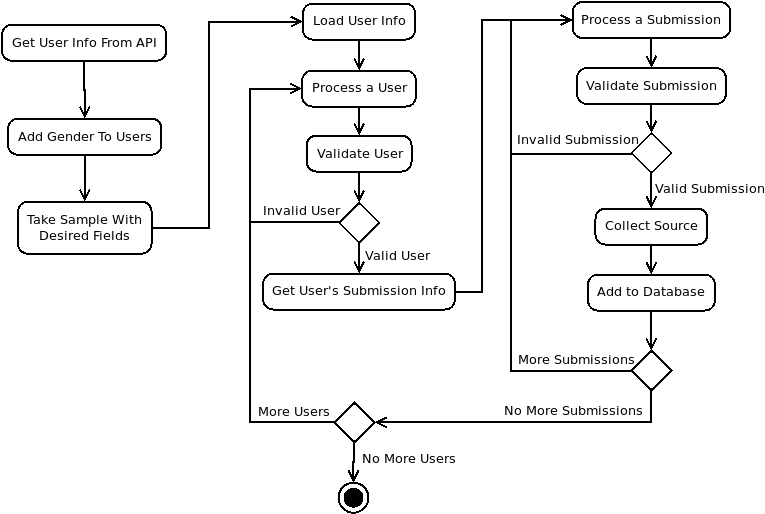
\includegraphics[height=8cm]{diagrams/cf_process.png}
    \caption{Getting Data From Codeforces}
\end{figure}


%% Discussion of each subprocess with technical details, the data collected, and the technical issues %%
\subsection{Process Details}
There are two processed used to collect the code. The most reliable is to use the Selenium web driver to open each users submission page to open popups that contain the source code and scrape it. The other way is to create links from user and submission records to a page that has the source code on it. These links seem work for short periods of time and then become unavailable for a slightly longer period. This makes it an unreliable method of collection to use on its own. Primarily collecting source code samples with the Selenium process and using links as a backup allows for most valid samples to be obtainable.

\subsubsection*{Process}
First a list of user records collected from the user records requested from the Codeforces API is loaded. Invalid user records are filtered out before the process is started so there is no need to validate the user records. For each user record a list of submission records is requested from the Codeforces API. When using Selenium only the most recent 50 submission records for a user are gathered because each page of submissions of Codeforces has 50 submissions per page. Only one submission for a problem is collected so a set of problem names for collected submissions is maintained. Before processing a user record the database is queried to add any previously collected problem names to this set.  The variations in submissions for the same problem are often minor for accepted solutions.

Before an attempt is made to collect source code for a submission it is validated. It must be an accepted solution for a problem that has not been collected for the current user. Team submissions are ignored as are non-programming submissions. It must also be written in one of the programming languages that is being collected.If a submission record does not meet these conditions then the process moves to the next submission.

The first attempt to collect the source code is done with the Selenium web driver. When the process starts a web browser is opened. For each user record the browser opens the users submissions page. On this page each submission's id is a link to open a popup containing the source code. The Selenium web driver can click this link and open the popup in the browser. Once the popup is open the pages html can be scraped and the source code is collected from it. Sometimes the submission id does not have a link available and the popup cannot be opened. When this happens another attempt is made using the second method.

The second attempt is made by taking some user, contest, and submission information and using it to construct a url. This url should lead to another page that has all the same information for the submission's source code. If this page is available to visit then its html is scraped and the source code collected from it. If the link does work and no source code can be obtained the process moves on to the next submission record.

If source code is collected it is added, along with selected information from the user and submission record, to the database. Each remaining submission record for the current user is processed. When all 50 submission records are processed, or a total of 50 submissions have been collected for the current user, next user record is processed.

When all user records are processed or a given limit for number of records to process is reached the process ends. Details on the range of records processed and the success rate for submissions and added source code samples are displayed.

\subsubsection*{Data}
Data is collected for the user and the submission. The required user information is Codeforces handle, first name, country, gender, gender probability, rank, and rating. All fields are strings except for gender probability which is a number between 0.0 and 1.0 and rating which is an integer. The handle is the users unique login name for Codeforces. The rank is a title that is given to users based on their overall ranking on the site. For example 'Expert' or 'Legendary Grand Master'. Rating is a number usually between 0 and 4000 and it determined the users overall ranking on the site. User information that may be present, but not required, is last name, city, organization, contribution, max rank, max rating, registration time. The first three are strings. contribution is a number and it has to do with a users activity in the Codeforces community. Max rank and max rating are the same as rank and rating, but represent the best of either the user has achieved. The registration time is a time stamp that indicates when the user signed up to codeforces.

All the submission information used is required except for problem difficulty which is not always available. The fields include a submission id, a problem name, a programming language, a participant type, and a submission time. Submission id is a unique integer identifier added to each submission by codeforces when the submission is made. The problem name is a string of the problem title. There are various participant types indicating what the user may have been doing when solving the problem. For example as a contestant or out of contests time. The time is a time stamp that is converted into integers for day, month, and year as well as a time string of the time of day. These new fields are stored in the database instead of the time stamp.

All Data collected from the API is in json format. It comes with more fields than are necessary for the process or for our research. Information on the API and additional fields can be found on the Codeforces website.

\begin{table}[t]
    \begin{center}
        \caption{Codeforces Data Fields}
        \label{tab:cf_data}
        \begin{tabular}{|l | c | c | c |}
            \hline
            \textbf{Field} & \textbf{Type} & \textbf{Required}\\
            \hline
            Handle & String & Yes\\
            First Name & String & Yes\\
            Last Name & String & No\\
            Gender & String & Yes\\
            Gender Probability & Float & Yes\\
            Country & String & Yes\\
            City & String & No\\
            Organization & String & No\\
            Contribution & String & No\\
            Rank & String & Yes\\
            Rating & Int & Yes\\
            Max Rank & String & No\\
            Max Rating & Int & No\\
            Registered & String & No\\
            \hline
            Submission id & Int & Yes\\
            Source Code & String & Yes\\
            Programming Language & String & Yes\\
            Problem Name & String & Yes\\
            Participant Type & String & No\\
            Time & String & No\\
            Year & Int & No\\
            Month & Int & No\\
            Day & Int & No\\
            \hline
        \end{tabular}
    \end{center}
\end{table}

\subsubsection*{Technical Issues}
There are some technical issues with using selenium. Because Selenium loads the pages in a web browser the process must wait for the page to load fully before it can continue. This means that there are some sleeps in the code for a couple seconds before scraping a popup and before clicking the next submission link after closing the popup. This slows down collection, but the failure rate is low so it is acceptable.

The codeforces web site can often be slow to load, and sometime become unresponsive. The process deals with this by reloading the page if it has failed to load after 30 seconds. This often solves the issue without too many refreshes, but it can waste a couple minutes. Sometimes Selenium cannot find the popup close button and the submission page must be refreshed to process the next submission. If it must be refreshed several times before it is ready again it can cause even more waiting.

In the end Selenium works very well, but it increases the complexity of the process and the components involved. This can make it hard to deal with all the errors that might come up while interacting with a web browser directly. It is difficult to guarantee that the process will run it for long periods of time unattended.

The constructed links not always working is an issue. It can be possible to collect 20 submissions and then fail to collect 50 or more. It seems to be a rather regular pattern, but it is not clear what causes it. The plus side is that only using these links is far less complicated and has been left running for days at a time. It may skip certain users or require some kind of sleep to make sure that it misses a minimum of submissions, but it might be acceptable if it could be left running 24 hours a day.



% Gender Labeling %%%%%%%%%%%%%%%%%%%%%%%%%%%%%%%%%%%%%%%%%%%%%%%%%%%%%%
\section{Adding Gender Labels}
Gender information is not available for users of GitHub or Codeforces. One of the common ways to add gender labels to user information is with the persons first name. There are a number of websites and APIs that offer gender data for first names. Most of them also allow for increased accuracy with the addition of country codes. There is evidence to suggest that these services can give an acceptable level of accuracy for the gendering of names, though the process is not without issues \cite{Santamaria2018}.

%% Introduction to the sources being used %%
\subsection{Data Source}
There are several available gender APIs, but the genderize.io was used for this to label our data. 'It utilizes big datasets of information, from user profiles across major social networks and exposes this data through its API' \cite{WEBSITE:GENDER1}. The API allows 1000 free name requests per day and is able to increase accuracy with added country data. All responses are stored in a local database to reduce the number of requests needed. The genderize.io service was used because it allows many more names to be gendered for free. It is also substantially cheaper than some of the other services. For a comparison of gender API rates see appendix A.

%% Discussion of the pros and cons and difficulties along with steps taken to try and overcome any issues. %%
\subsection{Pros And Cons}
\begin{itemize}
    \item \begin{sloppypar} This is essentially the only efficient way to add gender labels to programmers. Access to name data through country census data and birth name lists would be difficult to obtain. The results of various gender APIs have been shown to be more reliable than this kind of data \cite{Santamaria2018}. Also, trying to request gender data directly from programmers would not be feasible for any large dataset.\end{sloppypar}
    
    \item With several decent sources available for this kind of labeling it is possible to validate the results. When a set of samples is taken from the database gender could be requested from one or two of the other services. Samples that could not be agreed upon by all results could be discarded to improve the accuracy of the labels. Using a subset of the data would also reduce the cost of using services that require payment as opposed to trying to validate all the names at once.
    
    \item There are many common names in every country that show up in the data often. Keeping a local database of name and gender labels can significantly reduce the calls needed to an API over time.

    \item The probability given can help to determine the likelihood of results being correct, but it still is only as good as the service. Santamaria et al. present some benchmarks on the accuracy of several services including genderize.io \cite{Santamaria2018}.

    \item Most of the services offer some free requests, but other than genderize.io they are not enough for any serious use. They all offer payment options to increase limits, but can become expensive with a large number of requests.

    \item the possibility of programmers not providing their real names could be a problem. In order to get good results a country is needed. This can reduce the number of samples available for use.

    \item \begin{sloppypar} All services have been found to be less effective at labeling Asian names \cite{Santamaria2018}. This can present a problem for sources that have a large user base from Asian countries.\end{sloppypar}

    \item A name may have a high probability of being a certain gender, but the number of samples may be low which makes that accuracy questionable.
    
    \item These methods of gender labeling are firmly rooted in the gender binary and cultural naming conventions. The gender labels of names will be most likely to be connected to cultural norms and biological sex. Therefore they may not accurately represent the individual's gender.
\end{itemize}


%% Overview of the process %%
\subsection{Process Details}
\subsubsection*{Process}
A given name is looked up in the local database to see if the it has already been gendered. If the name has not already been gendered it is looked up with the genderize.io API. If no errors occur the name is added to the local database along with the returned gender information. If this process was called by another process a gender and gender probability are returned. Other processes are free to do what they need to with the results.

A country code was not used to gender the names in the dataset. When the collection started some of the details about the process were not fully understood. The quality of the gender data may be improved by verifying genders using country code. Once one has a dataset with desired samples the name and country code can be extracted and this list can be sent to one of the available APIs. The results can be used to re-gender the dataset or to confirm the accuracy of the previous gendering. For the highest accuracy it would probably be best to gender the samples with several APIs and keep those samples that were gendered the same by all of them.

\subsubsection*{Data}
The data consists of just the gender and the probability the gender label is correct. The gender is a string 'male', 'female', or 'null'. The probability is a float between 0.0 and 1.0. The Case of a name is ignored. There is also a 'count' field in the response that is described as 'the number of entries examined to calculate the result' \cite{WEBSITE:GENDER1}. If a country code was used it is also part of the response.

\begin{table}[t]
    \begin{center}
        \caption{Gender Data Fields}
        \label{tab:gen_data}
        \begin{tabular}{| l |c | c | c |}
            \hline
            \textbf{Field} & \textbf{Type} & \textbf{Values} & \textbf{Required}\\
            \hline
            Gender & String & {male, female, null} & Yes\\
            Probability & Float & [0.5, 1.0] & Yes\\ 
            Count & Int & [0, INF] & No\\
            Country Code & String & N/A & No\\
            \hline
        \end{tabular}
    \end{center}
\end{table}


% Database %%%%%%%%%%%%%%%%%%%%%%%%%%%%%%%%%%%%%%%%%%%%%%%%%%%%%%%%%%%%%
\section{Database}

Our database is setup with MySQL 8. The tables in the data section of each process show the schema for that process's database tables. Each GitHub collection process has separate tables for each programming language. For simplicity all table rows contain a string of source code and all the information about where that code came from and it's author. This is not the most efficient database setup, but it makes retrieving source code easy.

To work with the samples a query can be made to the database to select all rows that meet a certain set of conditions. These rows can be exported to csv or json and imported into whatever program or interpreter one is using. Once the records are imported they can be sorted or filtered to give desired groups. Most programming languages for data analysis have features that make this process simple compared to constructing complicated SQL queries to obtain a precise subset or grouping of the data. This also has the added benefit of loading all the data one might work with rather than making many queries and loading small subsets one at a time.

For Example the following SQL will collect all records from users in Canada.

\begin{singlespacing}
    \begin{verbatim}
        SELECT
            *
        FROM
            git_projects_py
        WHERE
            user_country_code='ca';
    \end{verbatim}
\end{singlespacing}
The results of this query. can be imported into a programming environment and grouped by gender or author. One could also loop through all the records and apply functions to each source code sample. This could be useful when creating feature vectors to use with machine learning algorithms.

Schemas for the database tables are listed in appendix B.


% Conclusion %%%%%%%%%%%%%%%%%%%%%%%%%%%%%%%%%%%%%%%%%%%%%%%%%%%%%%%%%%%
\section{Conclusions}
Using the processes described in this report it is possible to collect a large number of source code samples from GitHub and Codeforces. Our database contains more than 600,000 source code samples from over 100,000 distinct authors. It is also possible to add gender to these samples through the use of name APIs. This gendering process can have an acceptable level of accuracy if one is careful and chooses the right subset of data. The processes and dataset are tailored to the needs of sociolinguistic research, but could likely be used or adapted for other purposes as well.

\subsection{Threats To The Data Validity}
It may be possible to collect a large amount of data, it does not mean that it is all good data. We have taken steps to ensure that it meets our needs, but there are still some difficulties. With proper steps the effect of these difficulties could be reduces, but there will always be some margin of error.

\subsubsection*{Single Authors}
\begin{itemize}
    \item There are many third party libraries and other collections of code samples that people can add to GitHub projects. Our methods to use only files with single contributors cannot guarantee that the code added by that contributor was their own. Filtering out certain folders and files can help to reduce the possibility of this, but will not get all of them.
    \item Using git's blame feature works really great to get only single author files, but this assumes that the file was exclusively developed with git. If the project was added to git after it was created it is impossible to tell how many people contributed to it.
\end{itemize}

\subsubsection*{Contents of Samples}
\begin{itemize}
    \item The file could be too short.
    \item In some Codeforces samples templates are used to setup for a problem. This can make files seem longer, but may only contain a small amount of code written for the problem. The same kind of thing can be found with comments that begin files with license or other project information.
    \item Codeforces contest programming may differ substantially from more general purpose programming. This means that it may not be comparable to other kinds of code. For GitHub the same problem could arise from different problem domains. Especially if samples were short.
\end{itemize}

\subsubsection*{Gender Issues}
\begin{itemize}
    \item Each API has its own process for gendering names and it is not always clear what these methods are. Using more than one API and comparing results may help to improve results.
    \item All APIs have been shown to be less effective when gendering Asian names. This might not be as big a problem with GitHub because it is much more popular in the Europe and North America, but the Codeforces user base is overwhelmingly from countries like Russia, China, and India.
    \item If country is unavailable or unused the gender results from the APIs may not be as accurate.
    \item If gender results do not have high probabilities this could affect the accuracy of any predictions involving gender.
\end{itemize}


\subsection{Future Additions or Expansions}
\begin{itemize}
    \item Samples were only collected for three programming languages: Python, C++, and Java. The benefit of these languages is that they are all commonly used general purpose languages. There is a great deal of code available for each of them. They are also all procedural and object oriented programming languages. It might be worth collecting languages that are primarily functional or declarative languages. It could also be worthwhile to collect languages that are substantially different in syntax. Though it may be hard to find as many quality samples from languages that are less popular.
    \item The importance of country in gender labeling was not discovered until after a good portion of the data was collected. It would be valuable to either re-gender the data using country codes, or to build a process to consult other services to compare and refine the gender labels.
    \item It would also be valuable to find a process for removing contest templates or introductory comment sections from samples. Being able to automate the cleaning of the data in a reliable way would result in more time for analysis.
\end{itemize}


\newpage

\bibliography{technical_report}
\bibliographystyle{plain}


\newpage
\appendix

\section{Available Gender APIs}

Each gender service has different costs. The best for both free names and paid names is genderize.io. genderize, gender-api, and namsor all offer 1 name per credit. However, name-api offers a name per every 3 credits. So it's 10,000 free credits per month is only 3333 names. Also, the 100,000 credit per month price of \$55 would need to be multiplied by 3 to get the same number of names per month as the other services, but one would have to jump to the 1,000,000 credit per month tier which cost \$450/Month. The name-api service does offer paying for one time processing of batches of names, but these credits are more expensive.

\begin{sloppypar} For more information on accuracy and other benchmarks of these services see \textit{Comparison and benchmark of name-to-gender inference services} \cite{Santamaria2018}. \end{sloppypar}

\begin{table}[h!]
    \begin{center}
        \caption{Gender API comparison}
        \label{tab:gen_apis}
        \begin{tabular}{|l|c|c|}
            \hline
            \textbf{Service Url} & \textbf{Free Credits/Period} & \textbf{100,000 Credits/Month}\\
            \hline
            genderize.io & 1000/Day & \$9.00 \\
            gender-api.com & 500/Month & \$80.00 \\
            v2.namsor.com & 5000/Month & \$130.00 \\
            name-api.org & 10,000/Month & \$55.00 \\
            \hline
        \end{tabular}
    \end{center}
\end{table}

\newpage
\section{Database Schemas}
Each table shows the schema for one type of database table. Our database is split up into tables like 'git{\_}projects{\_}py' and 'git{\_}projects{\_}java', These tables share the same schema, but are separated by language.

\begin{table}[h!]
    \begin{center}
        \caption{Schema for GitHub Projects Tables}
        \label{tab:git_projects_schema}
        \begin{tabular}{|l | c | c |}
            \hline
            \textbf{Column Name} & \textbf{MySQL Type} & \textbf{Nullable}\\
            \hline
            id & int & PK\\
            user{\_}id & int & Yes\\
            user{\_}login & varchar & No\\
            user{\_}fullname & tinytext & No\\
            gender & varchar & No\\
            gender{\_}probability & float & No\\
            user{\_}company  & tinytext & Yes\\
            user{\_}created & tinytext & Yes\\
            user{\_}type & tinytext & Yes\\
            user{\_}country{\_}code & tinytext & No\\
            user{\_}state & tinytext & Yes\\
            user{\_}city & tinytext & Yes\\
            user{\_}location & tinytext & Yes\\
            \hline
            project{\_}id & int & UK\\
            project{\_}url & text & No\\
            project{\_}name & tinytext & Yes\\
            project{\_}language & tinytext & No\\
            project{\_}created & tinytext & Yes\\
            \hline
            file{\_}hash & varchar & UK\\
            file{\_}name & tinytext & No\\
            file{\_}contents & mediumtext & No\\
            file{\_}lines & int & No\\
            \hline
        \end{tabular}
    \end{center}
\end{table}

\begin{table}[h!]
    \begin{center}
        \caption{Schema for GitHub Commits Tables}
        \label{tab:git_commit_schema}
        \begin{tabular}{|l | c | c |}
            \hline
            \textbf{Column Name} & \textbf{MySQL Type} & \textbf{Nullable}\\
            \hline
            id & int & PK\\
            user{\_}id & int & Yes\\
            user{\_}login & varchar & No\\
            user{\_}fullname & tinytext & No\\
            gender & varchar & No\\
            gender{\_}probability & float & No\\
            user{\_}company  & tinytext & Yes\\
            user{\_}created & tinytext & Yes\\
            user{\_}type & tinytext & Yes\\
            user{\_}country{\_}code & tinytext & No\\
            user{\_}state & tinytext & Yes\\
            user{\_}city & tinytext & Yes\\
            user{\_}location & tinytext & Yes\\
            \hline
            project{\_}id & int & UK\\
            project{\_}url & text & No\\
            project{\_}name & tinytext & Yes\\
            project{\_}language & tinytext & No\\
            project{\_}created & tinytext & Yes\\
            \hline
            commit{\_}id & int & Yes\\
            commit{\_}sha & tinytext & No\\
            commit{\_}created & tinytext & Yes\\
            \hline
            file{\_}sha & varchar & UK\\
            file{\_}name & tinytext & No\\
            file{\_}contents & mediumtext & No\\
            file{\_}changes & int & No\\
            \hline
        \end{tabular}
    \end{center}
\end{table}

\begin{table}[h!]
    \begin{center}
        \caption{Schema for Codeforces Table}
        \label{tab:cf_schema}
        \begin{tabular}{|l | c | c |}
            \hline
            \textbf{Column Name} & \textbf{MySQL Type} & \textbf{Nullable}\\
            \hline
            handle & varchar & No\\
            first{\_}name & tinytext & No\\
            last{\_}name & tinytext & Yes\\
            gender & varchar & No\\
            gender{\_}probability & float & No\\
            country & tinytext & No\\
            city & tinytext & Yes\\
            organization & tinytext & Yes\\
            contribution & tinytext & Yes\\
            user{\_}rank & tinytext & No\\
            rating & int & No\\
            max{\_}rank & tinytext & Yes\\
            max{\_}rating & int & Yes\\
            registered & tinytext & Yes\\
            \hline
            submission{\_}id & int & PK\\
            source{\_}code & mediumtext & No\\
            programming{\_}language & varchar & No\\
            problem{\_}name & varchar & No\\
            participant{\_}type & tinytext & Yes\\
            time & tinytext & Yes\\
            year & int & Yes\\
            month & int & Yes\\
            day & int & Yes\\
            \hline
        \end{tabular}
    \end{center}
\end{table}

\begin{table}[h!]
    \begin{center}
        \caption{Schema For Gender Table}
        \label{tab:gen_schema}
        \begin{tabular}{| l |c | c |}
            \hline
            \textbf{Column Name} & \textbf{MySQL Type} & \textbf{Nullable}\\
            \hline
            name & String & No\\
            gender & String & No\\
            probability & Float & No\\
            \hline
        \end{tabular}
    \end{center}
\end{table}

\end{document}